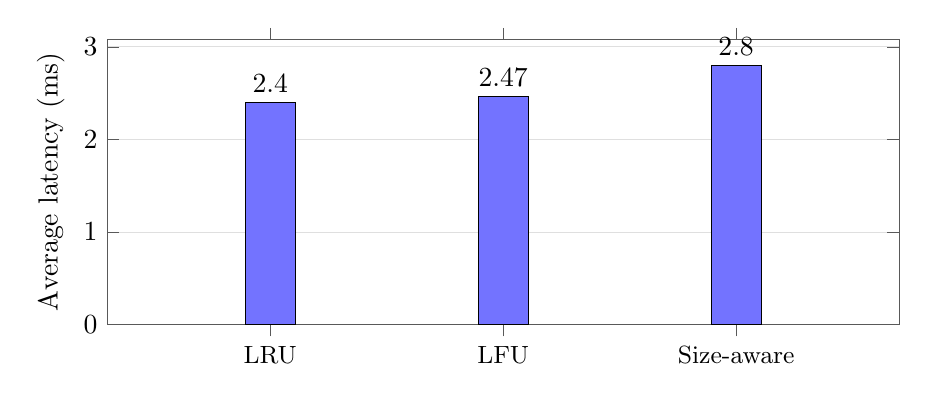
\begin{tikzpicture}
\begin{axis}[
  width=0.96\columnwidth,
  height=5.2cm,
  ybar,
  bar width=18pt,
  ymin=0,
  ylabel={Average latency (ms)},
  symbolic x coords={LRU,LFU,Size-aware},
  xtick=data,
  xticklabel style={font=\small},
  nodes near coords,
  nodes near coords align={vertical},
  enlarge x limits=0.35,
  major grid style={gray!25},
  axis line style={black!65},
  tick style={black!65},
  ymajorgrids=true
]
\addplot[fill=blue!55] coordinates {(LRU,2.401) (LFU,2.466) (Size-aware,2.797)};
\end{axis}
\end{tikzpicture}

\vspace{0.5em}

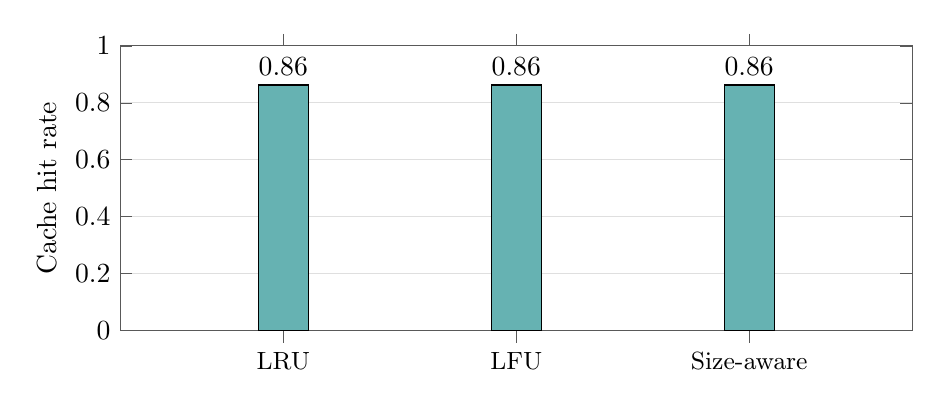
\begin{tikzpicture}
\begin{axis}[
  width=0.96\columnwidth,
  height=5.2cm,
  ybar,
  bar width=18pt,
  ymin=0,
  ymax=1.0,
  ylabel={Cache hit rate},
  symbolic x coords={LRU,LFU,Size-aware},
  xtick=data,
  xticklabel style={font=\small},
  nodes near coords,
  nodes near coords align={vertical},
  enlarge x limits=0.35,
  major grid style={gray!25},
  axis line style={black!65},
  tick style={black!65},
  ymajorgrids=true
]
\addplot[fill=teal!60] coordinates {(LRU,0.8625) (LFU,0.8625) (Size-aware,0.8625)};
\end{axis}
\end{tikzpicture}
